\section{metodi risolutivi}

Una tipologia di equazioni differenziali che abbiamo già trattato
è data dalle equazioni della forma:
\[
   u'(x) = f(x).
\]
Banalmente l'insieme delle soluzioni è dato dalle primitive di $f$:
\[
  u \in \int f.
\]
Se $f$ è definita su un intervallo tutte le soluzioni sono definite sullo stesso
intervallo e, grazie al Teorema~\ref{th:primitive}
si scrivono quindi nella forma
\[
  u(x) = F(x) + c
\]
dove $F$ è una qualunque primitiva di $f$ e $c\in \RR$ è una costante additiva
arbitraria.
Se $f$ è continua e consideriamo il problema di Cauchy:
\[
  \begin{cases}
    u'(x) = f(x) \\
    u(x_0) = y_0.
  \end{cases}
\]
possiamo identificare una unica soluzione
che si scrive nella forma:
\[
  u(x) = y_0 + \int_{x_0}^x f(t)\, dt.
\]

\subsection{equazioni lineari del primo ordine}

Le equazioni differenziali ordinarie del primo
ordine in forma normale possono essere scritte nella forma:
\mymark{***}
\begin{equation}\label{eq:47744}
   u'(x) + a(x) u(x) = b(x).
\end{equation}

Per risolvere queste equazioni si cerca di ricondurre la somma
nel lato sinistro alla derivata di un prodotto.
Per fare ciò si considera una qualunque primitiva
$A\in \int a$ e si moltiplicano ambo i membri
per $e^{A(x)}$:
\[
  e^{A(x)} u'(x) + a(x) e^{A(x)} u(x) = b(x) e^{A(x)}
\]
essendo $A'(x) = a(x)$
si osserva che il lato sinistro è ora la derivata di un prodotto:
\[
  \enclose{e^{A(x)}u(x)}' = b(x) e^{A(x)}
\]
da cui
\[
  e^{A(x)} u(x) \in \int b(x) e^{A(x)}\, dx.
\]
Moltiplicando ambo i membri per $e^{-A(x)}$ (visto che l'esponenziale
non si annulla mai questa operazione non modifica lo spazio delle soluzioni)
si ottiene
\[
u(x) = e^{-A(x)} \int b(x) e^{A(x)}\, dx, \qquad
A(x) \in \int a(x)\, dx.
\]

Più esplicitamente
scelta una qualunque primitiva del lato destro
\[
  F(x) \in \int b(x) \cdot e^{A(x)}\, dx
\]
su ogni intervallo in cui $a(x)$ e $b(x)$ sono definite
si ha
\[
  u(x) = e^{-A(x)}\cdot \enclose{F(x) + c}.
\]
per qualche $c\in \RR$.

Se $b(x)=0$ l'equazione è lineare omogenea, possiamo scegliere $F(x) = 0$
e quindi lo spazio delle soluzioni in questo caso
è dato da
\[
  u(x) = c \cdot e^{-A(x)}
\]
ed è quindi lo spazio vettoriale unidimensionale generato dalla funzione $e^{-A(x)}$.

Ogni soluzione della equazione non omogenea si può scrivere come somma di una
soluzione particolare $u_0$ della equazione non omogenea
più una generica soluzione dell'equazione omogenea associata. Infatti:
\[
  u(x) = u_0(x) + c e^{-A(x)}
\]
dove
\[
  u_0(x) = e^{-A(x)}F(x)
\]
è una particolare soluzione dell'equazione non omogenea.

Osserviamo che se $a(x)$ e $b(x)$ sono funzioni continue definite su uno stesso
intervallo $I$, anche la soluzione è definita su tutto $I$.
Si dirà quindi che la soluzione esiste \emph{globalmente}.

\begin{exercise}[autovettori dell'operatore derivata]%
  \label{ex:58230978}
Fissato $\lambda \in \RR$ trovare tutte le soluzioni dell'equazione
\[
  u'(x) = \lambda u(x).
\]
\end{exercise}
%
\begin{proof}[Svolgimento]
Scriviamo l'equazione nella forma
\[
  u'(x) - \lambda u(x) = 0.
\]
Nelle notazioni precedenti abbiamo $a(x) = -\lambda$ e quindi possiamo scegliere $A(x) = -\lambda x \in \int a$.
Moltiplicando ambo i membri per $e^{A(x)}$ si ottiene
\[
  e^{-\lambda x} u'(x) - \lambda e^{-\lambda x} u(x) = 0
\]
cioè
\[
 \enclose{e^{-\lambda x}\cdot u(x)}' = 0
\]
da cui su ogni intervallo in cui $u$ è definita esiste una costante $c$ tale che
\[
  e^{-\lambda x} u(x) = c
\]
ovvero
\[
  u(x) = c e^{\lambda x}.
\]
Abbiamo dunque trovato che le soluzioni sono definite su tutto $\RR$, una soluzione è $e^{\lambda x}$ e ogni altra soluzione è multiplo di questa.
\end{proof}

\begin{exercise}
\begin{enumerate}
\item
Trovare le soluzioni dell'equazione differenziale
\[
  u' - \frac{u}{x} = x^2.
\]

\item
Trovare le soluzioni dell'equazione differenziale
\[
  x u' - u = x^3.
\]
\end{enumerate}
\end{exercise}
\begin{proof}[Svolgimento]
La prima è una equazione lineare non omogenea del primo ordine
del tipo~\eqref{eq:47744}. Il fattore integrante è $e^{A(x)}$ con
\[
  A(x) \in \int a(x)\, dx = -\int \frac{1}{x}\, dx \ni - \ln \abs{x}.
\]
Dunque $e^{A(x)} = 1/\abs{x}$. Dovremmo dunque dividere ambo i membri dell'equazione per $\abs{x}$. Osserviamo che l'equazione non è definita per $x=0$ e possiamo dunque distinguere i casi $x>0$ e $x<0$. Decidiamo quindi, per semplicità, di cambiare segno all'equazione per $x<0$ cosicché possiamo dividere per $x$ invece che per $\abs{x}$.
Si ottiene dunque:
\[
  \frac{u'}{x} - \frac{u}{x^2} = x
\]
cioè
\[
  \enclose{u\cdot \frac{1}{x}}'  = x
\]
da cui
\[
  \frac{u}{x} \in \int x\, dx \ni \frac{x^2}{2}.
\]
Dunque la funzione $u(x)/x$ differisce da $x^2/2$ per una costante su ognuno dei due intervalli $x>0$ e $x<0$. Su ognuno dei due intervalli si ha dunque:
\[
  \frac{u(x)}{x} = \frac{x^2}{2} + c
\]
da cui
\[
  u(x) = \frac{x^3}{2} + c x
\]
per qualche $c\in \RR$. Per come è stato posto il problema, la soluzione non deve essere definita per $x=0$ e la costante $c$ può essere quindi diversa se $x>0$ o $x<0$.

La seconda equazione è equivalente alla prima se $x\neq 0$. Ma non è in forma normale e le soluzioni
potranno essere definite anche per $x=0$.
Si avrà quindi
\[
  u(x) = \frac{x^3}{2} + c x
\]
come prima ma affinché la funzione sia derivabile in $x=0$ la costante $c$ dovrà essere uguale per $x>0$ e per $x<0$.

Si osservi che ogni soluzione soddisfa la condizione iniziale $u(0) = 0$ 
e che quindi nessuna soluzione soddisfa la condizione $u(0)= q$ se $q \neq 0$.
\end{proof}

\begin{exercise}
Risolvere l'equazione differenziale:
\[
 u' + \frac{u}{(1+x^2)\arctg x} = 1.
\]
\end{exercise}
%
\begin{proof}[Svolgimento.]
Osserviamo che l'equazione è definita solo per $x\neq 0$. Cercheremo quindi le soluzioni sui due intervalli $x<0$ e $x>0$.
Moltiplicando ambo i membri dell'equazione per $\arctg x$ si ottiene
\[
  \arctg x \cdot u'(x) +\frac{1}{1+x^2} u(x) = \arctg x
\]
cioè:
\[
  \enclose{\arctg x \cdot u(x)}' = \arctg x
\]
da cui
\[
  \arctg x \cdot u(x) \in \int \arctg x\, dx \ni x \arctg x - \frac {1}{2}\ln(1+x^2).
\]
Dunque su ogni intervallo su cui la soluzione è definita esisterà
$c\in \RR$ tale che
\[
  \arctg x \cdot u(x) = x \arctg x - \frac{1}{2}\ln(1+x^2) + c
\]
da cui essendo $x\neq 0$ si può dividere per $\arctg x$ e ottenere
\[
  u(x) = x - \frac{\ln(1+x^2)}{2\arctg x} + \frac{c}{\arctg x}.
\]
Abbiamo quindi una famiglia di soluzioni definite per $x<0$ e una famiglia di soluzioni definite per $x>0$.
\end{proof}

\subsection{equazioni a variabili separabili}

Si chiamano equazioni a variabili separabili le
equazioni del tipo:
\mymark{***}
\begin{equation}\label{eq:edo_separabile}
  u'(x) = f(x) \cdot g(u(x)).
\end{equation}
Questa è una equazione del primo ordine in forma normale:
\[
  u'(x) = F(x, u(x))
\]
dove nella funzione $F$ risulta possibile separare le
due variabili in un prodotto:
\[
  F(x, y) = f(x)\cdot g(y).
\]

Se $u$ è una soluzione dell'equazione~\eqref{eq:edo_separabile}
e se $x$ è un punto in cui $g(u(x))\neq 0$, possiamo dividere ambo i membri dell'equazione per $g(u(x))$ per ottenere:
\[
  \frac{u'(x)}{g(u(x))} = f(x).
\]
Vogliamo ora scrivere il lato sinistro come la derivata della funzione composta. Se scegliamo una primitiva di $1/g$:
\[
  H(u) \in \int \frac{1}{g(u)}\, du
\]
si osserva che
\[
  \enclose{H(u(x))}' = H'(u(x))\cdot u'(x) = \frac{u'(x)}{g(u(x))} = f(x).
\]
dunque se $F\in \int f$, su ogni intervallo in cui $g(u(x))\neq 0$ dovrà esistere $c\in \RR$ tale che
\[
  H(u(x)) = F(x) + c.
\]
Se supponiamo inoltre che $H$ sia invertibile si avrà:
\[
  u(x) = H^{-1}(F(x)+ c).
\]

\begin{example}
Risolviamo l'equazione 
\begin{equation}\label{eq:separabile}
  u' = x^2 e^u.
\end{equation}
\end{example}
%
\begin{proof}[Svolgimento.]
Visto che $e^u \neq 0$ possiamo dividere ambo i membri dell'equazione 
per $e^u$:
\[
  \frac{u'(x)}{e^{u(x)}} = x^2  
\]
prendendo le primitive di ambo i membri otteniamo
\[
 \int\frac{u'(x)}{e^{u(x)}}\, dx  = \int x^2\, dx 
\]
e facendo il cambio di variabili: $u=u(x)$, $du = u'(x) dx$ 
otteniamo:
\[
  \Enclose{\int e^{-u}\, \, du}_{u=u(x)} = \frac{x^3}{3} + c
\]
da cui 
\[
  -e^{-u(x)} = \frac{x^3}{3} + c
\]
ovvero $u(x) = -\ln\enclose{-c -  \frac{x^3}{3}}$.
Posto $b=-c$
si ottiene 
\[
  u(x) = -\ln \enclose{b-\frac{x^3}{3}}.
\]
Dunque per ogni $b\in \RR$ si ottiene una soluzione 
$u\colon \openinterval{-\infty}{\sqrt[3]{3b}}\to \RR$.
\end{proof}
%
\newsavebox{\qrseparabile}\sbox{\qrseparabile}{%
\myqrshortdoclink{separabile}{i grafici delle soluzioni dell'equazione differenziale (\getrefnumber{eq:separabile})}}
\begin{figure}
\centering
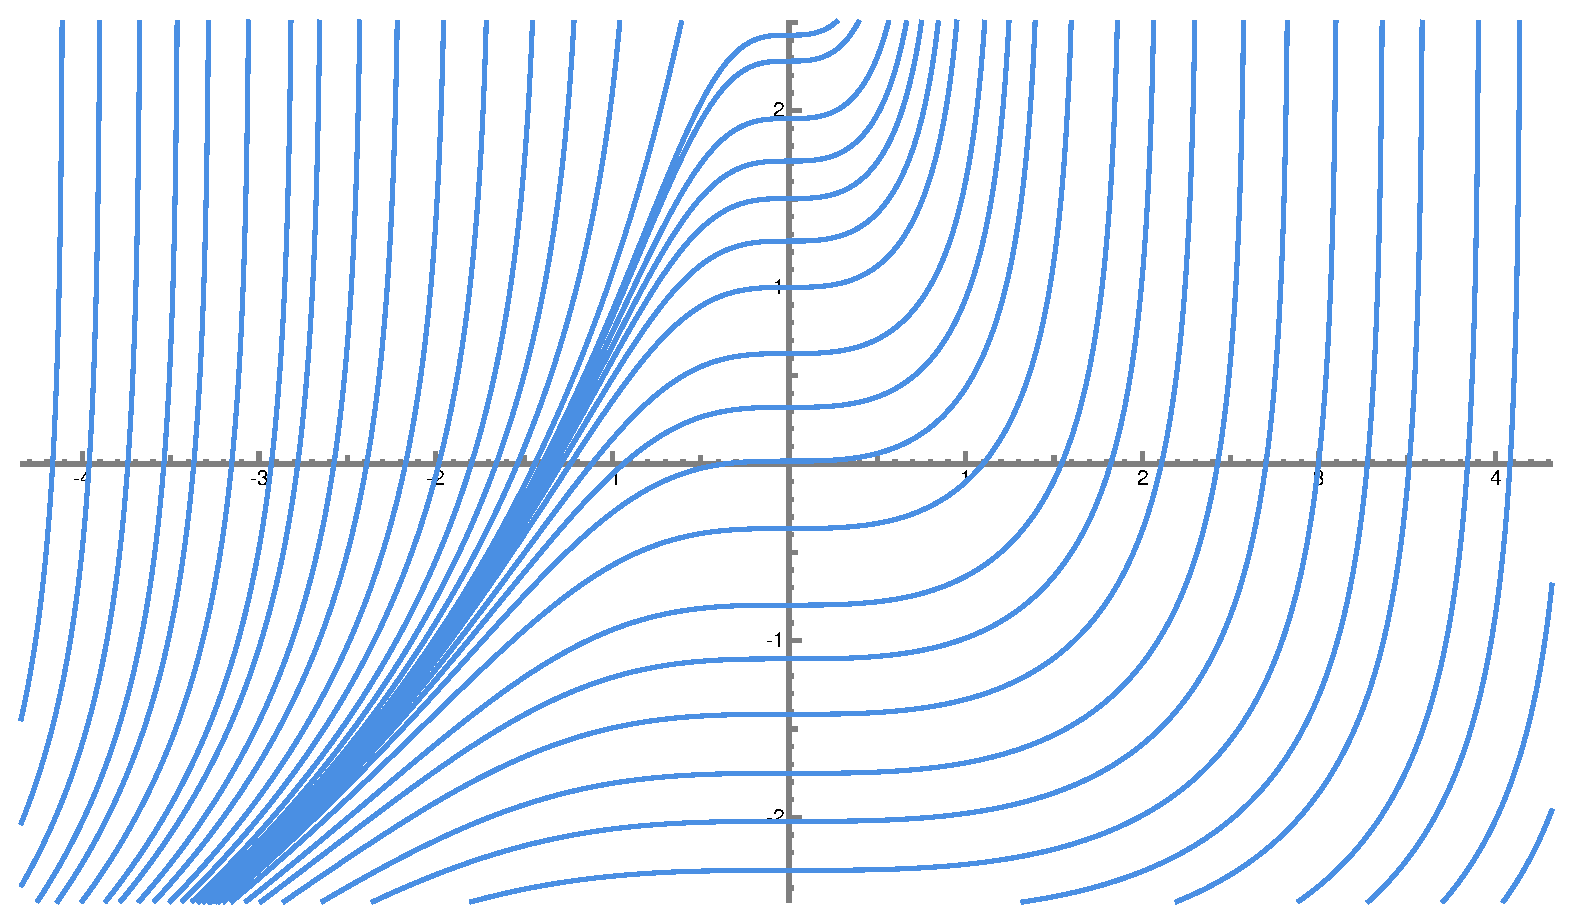
\includegraphics[width=0.8\textwidth]{fig_edo_separabile.pdf}
\caption{i grafici delle soluzioni dell'equazione differenziale~\eqref{eq:separabile}.
Si noti che ogni soluzione ha un asintoto verticale, dunque le singole 
soluzioni non sono definite su tutto $\RR$.
Ma scelto un qualunque punto del piano c'è una soluzione che passa per 
quel punto e inoltre due diverse soluzioni non si incontrano mai.
Queste proprietà sono garantite dal teorema~\ref{th:banach-caccioppoli}.
\ifwidemargin\\\\\fi%
\usebox{\qrseparabile}}
\label{fig:separabile}
\end{figure}

\begin{example}
Risolviamo l'equazione
\begin{equation}\label{eq:43856}
  u' = x u^2 + x.
\end{equation}
\end{example}
%
\begin{proof}[Svolgimento.]
E' una equazione del primo ordine in forma normale.
Raccogliendo $x$ al lato destro si ottiene una equazione a variabili separabili.
Dividendo ambo i membri per $u^2+1$ (che è sempre diverso da zero) si ottiene l'equazione equivalente
\[
\frac{u'}{1+u^2} = x.
\]
Integrando il lato sinistro si ottiene:
\[
  \int \frac{u'(x)}{1+u^2(x)}\, dx
  = \Enclose{\int \frac{du}{1+u^2}}_{u=u(x)}
  \ni \arctg(u(x))
\]
mentre per il lato destro si ottiene
\[
  \int x\, dx \ni \frac{x^2}{2}.
\]
Dunque su ogni intervallo si deve avere
\[
  \arctg(u(x)) = \frac{x^2}{2} + c.
\]
Visto che l'arcotangente assume valori compresi tra $-\pi/2$ e $\pi/2$ anche il lato destro dovrà rimanere in tale intervallo. Dovrà quindi essere:
\begin{equation}\label{eq:4856}
  -\frac \pi 2 < \frac {x^2} 2 + c < \frac \pi 2 .
\end{equation}
Con questa condizione possiamo invertire l'arcotangente ottenendo finalmente una espressione per la soluzione:
\begin{equation}\label{eq:45876314}
  u(x) = \tg\enclose{\frac{x^2}{2} + c}.
\end{equation}

\newsavebox{\qrquattrotre}\sbox{\qrquattrotre}{%
\myqrshortdoclink{43856}{i grafici delle soluzioni dell'equazione differenziale (\getrefnumber{eq:43856})}}
\begin{figure}
\centering
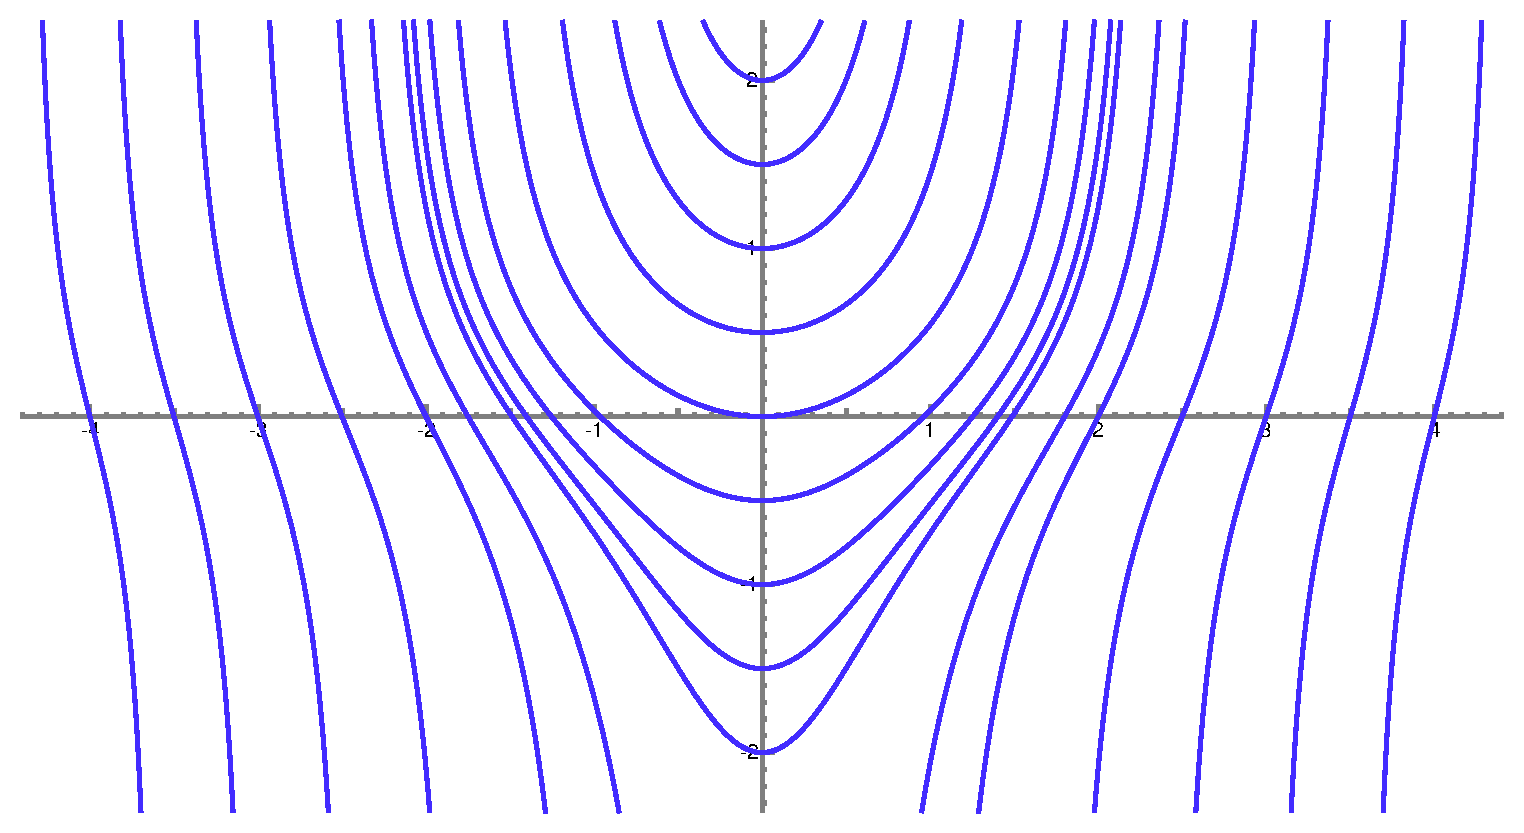
\includegraphics[width=0.8\textwidth]{fig_43856.pdf}
\caption{i grafici delle soluzioni dell'equazione differenziale~\eqref{eq:43856}.
\ifwidemargin\\\\\fi%
\usebox{\qrquattrotre}}
\label{fig:43856}
\end{figure}

Osserviamo che la condizione~\eqref{eq:4856} equivale a richiedere che l'argomento
della tangente stia nell'intervallo $\enclose{-\frac \pi 2, \frac \pi 2}$.
In tal caso dovrà essere $c<\frac\pi 2$ e si osserva che se $c>-\frac \pi 2$
la soluzione $u(x)$ è definita su un intervallo aperto centrato in $x=0$ mentre
se $c \le -\frac \pi 2$ la soluzione è definita su una coppia di intervalli
simmetrici con ampiezza che tende a zero quando $c\to -\infty$.
Agli estremi di tali intervalli la soluzione ha degli asintoti verticali.

In questo caso possiamo osservare che la condizione~\eqref{eq:4856} può essere
trascurata, visto che la funzione $\tg$ è $\pi$-periodica e quindi
è possibile sommare a $c$ un multiplo intero di $\pi$ senza che la soluzione
venga modificata.
Nell'equazione~\eqref{eq:45876314} si potrebbe
quindi considerare la funzione $\tg$
definita su tutto il suo dominio osservando che in tal caso si può
supporre che sia $c\in \left(-\frac \pi 2, \frac \pi 2\right]$.
Invece di ottenere un singolo intervallo per ogni $c$ si ottengono così
tutti gli infiniti intervalli.
\end{proof}

\begin{remark}
L'esempio precedente mette in evidenza il fatto che le soluzioni massimali possono essere definite
su intervalli arbitrariamente piccoli anche se l'equazione differenziale
non presenta singolarità. Diremo in questo caso che
la soluzione non è globale.

D'altra parte si osserva che i grafici delle soluzioni riempiono tutto il piano senza 
mai toccarsi l'uno con l'altro (si dice a volte che sono una \emph{fibrazione}).
Questo è dovuto al fatto che questa equazione soddisfa il 
teorema~\ref{th:cauchy_lipschitz} e quindi per ogni punto 
del piano passa una ed una sola soluzione.
\end{remark}

\begin{example}
Si voglia risolvere l'equazione
\[
  u' = u^2.
\]
Si tratta di una equazione in forma normale, del primo ordine, autonoma.
In particolare è a variabili separabili
$u' = f(u(x))\cdot g(x)$
con $f(u)=u^2$ e $g(x)=1$.
Osserviamo innanzitutto che $u(x) = 0$ è soluzione in quanto $u'(x) = u^2(x) = 0$.
Se $u$ è una soluzione non identicamente nulla ci saranno dei punti in cui
$u(x)\neq 0$.
In un intorno di tali punti possiamo dividere ambo i membri dell'equazione per $u^2(x)$ ottenendo:
\[
  \frac{u'}{u^2} = 1.
\]
Integrando il lato sinistro tramite cambio di variabile $u=u(x)$, $du=u'(x)\, dx$ si ottiene:
\[
  \int \frac{u'(x)}{u^2(x)}\, dx = \Enclose{\int \frac{du}{u^2}}_{u=u(x)} = \Enclose{-\frac{1}{u}}_{u=u(x)}
  = -\frac{1}{u(x)}
\]
mentre integrando il lato destro si ha
\[
  \int 1 \, dx \ni x.
\]
Dunque su ogni intervallo in cui $u(x)\neq 0$ deve esistere una costante $c\in \RR$ tale che
\[
-\frac{1}{u(x)} = x + c
\]
ovvero, ponendo $x_0 = -c$
\begin{equation}\label{eq:5782196}
  u(x) = -\frac{1}{x+c} = \frac{1}{x_0-x}.
\end{equation}

In conclusione abbiamo trovato una soluzione costante $u(x)=0$ e una famiglia
di soluzioni definite sugli intervalli $(-\infty,x_0)$ e $(x_0,+\infty)$
rappresentante dall'equazione~\eqref{eq:5782196}.
Dovremmo ora chiederci
se è possibile che queste soluzioni vengano mescolate tra loro, ovvero
se una soluzione può valere zero in alcune zone e soddisfare~\eqref{eq:5782196}
in altre.

In questo caso la risposta è no.
Basta osservare che una funzione $u$ che soddisfa l'equazione~\eqref{eq:5782196}
può tendere a zero solamente quando $x\to +\infty$ o $x\to -\infty$.
Questo significa che se consideriamo una soluzione $u(x)$
definita su un intervallo $I$ e se in almeno un punto la soluzione è diversa da zero,
allora la soluzione è diversa da zero su tutto $I$ e
soddisfa l'equazione~\eqref{eq:5782196} in quanto la soluzione nulla e la
soluzione \eqref{eq:5782196} non sono tra loro compatibili (non possono essere
incollate con continuità).

Vedremo più avanti un risultato
(proposizione~\ref{prop:separazione_soluzioni})
che garantisce in ipotesi molto generali che due diverse soluzioni non
possono mai incontrarsi.
\end{example}

\begin{exercise}
Fissato $p>1$ si risolva l'equazione differenziale
\[
  u' = u^p
\]
e si osservi che la soluzione presenta sempre un asintoto verticale
(dunque non c'è esistenza globale).
\end{exercise}

\begin{example}[baffo di Peano]
Si determinino tutte le soluzioni del problema di Cauchy
\begin{equation}
\label{eq:94467}
\begin{cases}
  u'(x) = \sqrt[3]{u(x)}\\
  u(0)=0
\end{cases}
\end{equation}
\end{example}
%
\newsavebox{\qrnovequattro}\sbox{\qrnovequattro}{%
\myqrshortdoclink{94467}{Il baffo di Peano formato dalle soluzioni del problema di Cauchy (\getrefnumber{eq:94467})}}
\begin{figure}
\centering
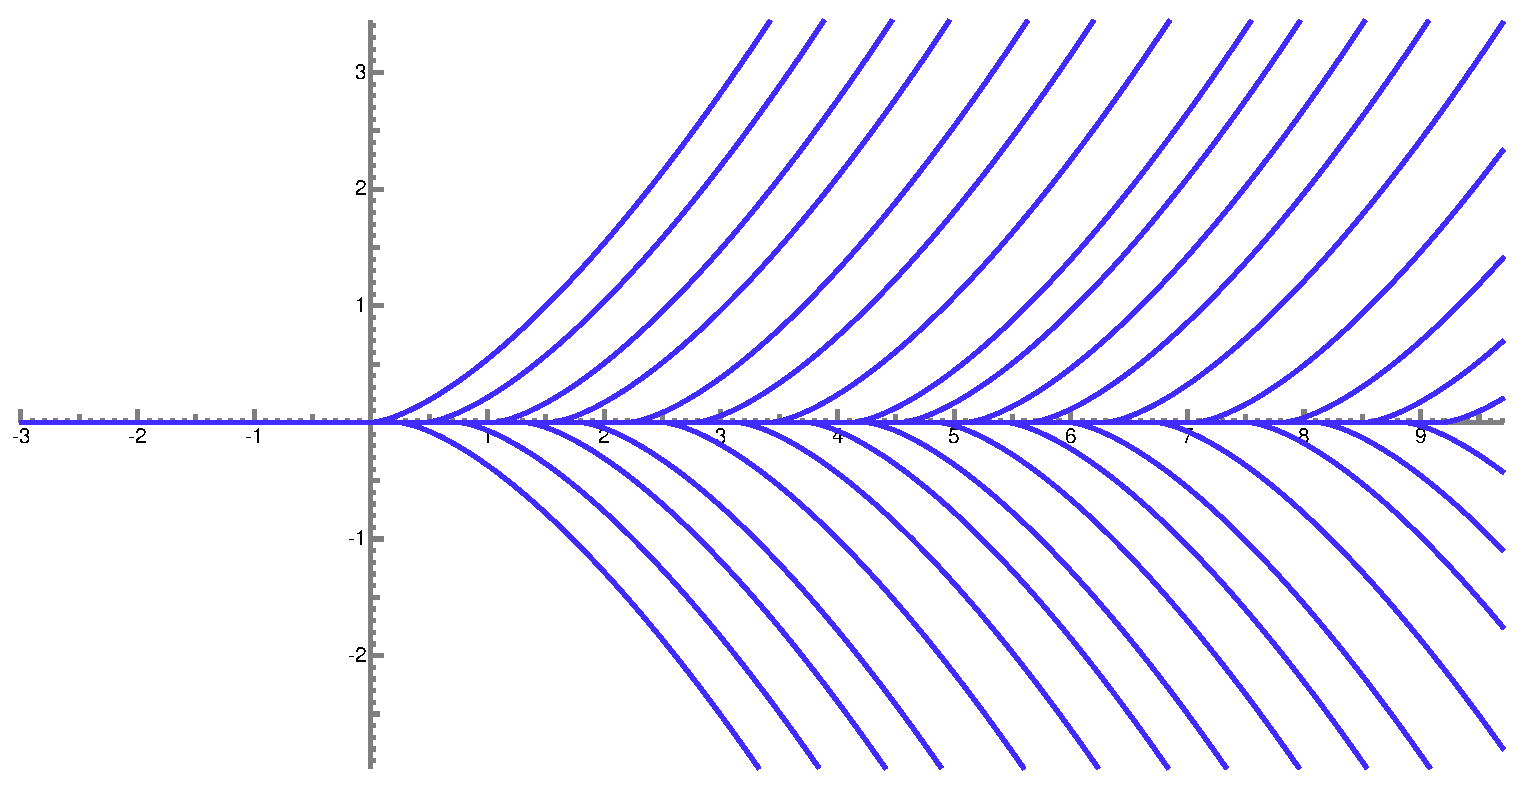
\includegraphics[width=0.9\textwidth]{fig_94467.pdf}
\caption{Il baffo di Peano formato dalle soluzioni del problema di Cauchy~\eqref{eq:94467}.\\\\
\usebox{\qrnovequattro}}
\label{fig:94467}
\end{figure}
%
\begin{proof}[Svolgimento.]
Osserviamo che la funzione nulla $u(x)=0$ è soluzione dell'equazione
e soddisfa la condizione $u(0)=0$.
Ma a priori non possiamo escludere che ci siano altre soluzioni dell'equazione
che verifichino la stessa condizione (vedremo che la
proposizione~\ref{prop:separazione_soluzioni} non si applica in questo caso
particolare).

Nei punti in cui $u(x)\neq 0$ possiamo riscrivere l'equazione nella forma
\[
  \frac{u'(x)}{\sqrt[3]{u(x)}} = 1.
\]
Integrando il lato sinistro tramite il cambio di variabili $u=u(x)$,
$du = u'(x)\, dx$,
si ottiene
\[
  \int \frac{u'(x)}{\sqrt[3]{u(x)}}\, dx
  = \Enclose{\int \frac{du}{\sqrt[3]u}}_{u=u(x)}
  \ni \frac 3 2 \sqrt[3]{u^2(x)}.
\]
integrando anche il lato destro troviamo dunque
che su ogni intervallo su cui $u$ è definita e $u(x)\neq 0$
deve esistere una costante $c$ tale che
\[
  \frac 3 2 \sqrt[3]{u^2(x)} = x + c.
\]
Risolvendo in $u(x)$:
\begin{equation}\label{eq:476937568}
  u(x) = \pm \sqrt{\enclose{\frac 2 3 (x+c)}^3}.
\end{equation}
Osserviamo che la proprietà precedente
può essere soddisfatta solamente se $x\ge -c$ ma affinché
sia $u(x)\neq 0$ dobbiamo imporre $x>-c$.
Ma per $x\to -c^+$
si ha $u(x)\to 0$ e anche $u'(x) = \sqrt[3]{u(x)}\to 0$.
Significa che una soluzione definita su $x>c$ mediante
la~\eqref{eq:476937568} può essere estesa a tutto $\RR$
ponendo $u(x)=0$ per $x\le c$.
Affinché valga la condizione $u(0)=0$ sarà dunque sufficiente
imporre la restrizione $-c\ge 0$.

Il nostro problema ha dunque infinite soluzioni definite
su tutto $\RR$. Per la precisione, per ogni $c\ge 0$
(cambiamo segno alla costante trovata prima, in modo che risulti
positiva)
si hanno le soluzioni
\[
  u(x) = \begin{cases}
    0 & \text{per $x\le c$}\\
    \sqrt{\enclose{\frac 2 3 (x-c)}^3} & \text{per $x>c$}
  \end{cases}
\]
e
\[
  u(x) = \begin{cases}
    0 & \text{per $x\le c$}\\
    -\sqrt{\enclose{\frac 2 3 (x-c)}^3} & \text{per $x>c$}
  \end{cases}
\]
\end{proof}
\subsection{altri metodi risolutivi}

Nella sezione precedente abbiamo visto che le equazioni lineari del primo ordine
e le equazioni
a variabili separabili possono essere ricondotte al calcolo di una primitiva.
Nella sezione~\ref{sec:edo_lineari} verranno esposti i metodi risolutivi per le
equazioni lineari di ordine $n$ a coefficienti costanti.

Ci sono molti altri tipi di equazioni che possono essere ricondotti
alle equazioni lineari o alle equazioni a variabili separabili.
Non potremo dilungarci su questi metodi ma può essere utile,
come riferimento non esaustivo,
un elenco di alcune tipologie di equazioni per le quali esiste un metodo
risolutivo.

\begin{enumerate}
\item \emph{Equazione del secondo ordine senza dipendenza da $u$}
\[
  F(x, u', u'') = 0
\]
si riconduce al primo ordine ponendo $u'(x) = v(x)$, $u''(x) = v'(x)$.

\item \emph{Equazione del secondo ordine autonoma}
\[
  F(u, u', u'') = 0
\]
si riconduce al primo ordine
ponendo $u'(x) = v(u(x))$,
$u''(x) = v'(u(x))\cdot v(u(x))$.

\item \emph{Equazioni del primo ordine omogenee}
\index{equazione!omogenea}%
\[
  u' = h(x,u(x))
\]
dove $h$ è omogenea, cioè: $h(tx,ty)=h(x,y)$ per ogni $t\in \RR$.
Si riconduce ad una equazione a variabili separabili facendo 
la sostituzione $u(x) = x\cdot v(x)$.

\item \emph{Equazione di Bernoulli}
\index{equazione!di Bernoulli}%
\index{Bernoulli!equazione di}%
\[
  u' = a(x) u + b(x) u^\alpha
\]
si riconduce ad una equazione lineare dividendo tutto per $u^\alpha$
e ponendo $u(x)^{1-\alpha} = v(x)$, $\frac{u'}{u^\alpha} = \frac{v'}{1-\alpha}$.

\item \emph{Equazione di Clairaut}
\index{equazione!di Clairaut}%
\index{Clairaut!equazione di}%
\[
  u = x u' + f(u');
\]
derivando l'equazione si ottiene $ u' = u' + xu'' + f'(u')u''$
che si fattorizza: $u''\cdot(x+f'(u'))=0$. 
Il secondo fattore ci permette di determinare $u'(x)$ e inserendo $u'$
nell'equazione originaria troviamo $u(x)$. 
Il primo fattore $u''=0$ ci dà come soluzione una retta che, sostituendone 
l'equazione nella equazione originaria, scopriamo essere tangente 
alla soluzione trovata precedentemente.
A queste soluzioni bisogna aggiungere le soluzioni non $C^2$ formate da un tratto
della curva inizale e che poi si staccano lungo le semirette tangenti.

\item \emph{equazione di Riccati}
\index{equazione!di Riccati}%
\index{Riccati!equazione di}%
\[
  u' = u^2 + b(x) u + c(x).
\]
si ponga $u(x) = -v'(x)/v(x)$ per ricondursi ad
una equazione lineare del secondo ordine in $v$:
\[
 v'' -  b(x) v' + c v = 0.
\]
\end{enumerate}

\begin{example}[equazione di Newton]
\index{equazione!di Newton}%
\index{Newton!equazione di}%
Un sistema fisico unidimensionale soggetto a forze che dipendono solamente
dalla posizione può essere descritto da un problema di Cauchy:
\[
\begin{cases}
  u''(x) = F(u(x)) \\
  u(x_0) = u_0 \\
  u'(x_0) = v_0
\end{cases}
\]
(ad esempio per il pendolo si ha $F(y) = -\sin y$).
La funzione $v$ definita da $v(u(x)) = u'(x)$ mette in relazione
la velocità con la posizione e descrive quindi il moto nel
cosiddetto \emph{spazio delle fasi}. Con tale sostituzione si
trova
\[
  u''(x) = v'(u(x)) u'(x) = v'(u(x)) v(u(x))
\]
che sostituita in $u'' = F(u)$ ci dà una equazione
differenziale del primo ordine per $v=v(u)$:
\[
 v' v  = F(u).
\]
Questa è una equazione del primo ordine a variabili separabili
che può essere interpretata come la legge di conservazione dell'energia,
infatti è equivalente a
\[
  \frac{d}{dx}\enclose{\frac 1 2 v^2 - \int F(u)} = 0
\]
dove $\frac 1 2 v^2$ si interpreta come energia cinetica e $-\int F$
come energia potenziale.
Integrando tra $x_0$ e $x$ e utilizzando le condizioni iniziali si ottiene,
con $u=u(x)$:
\[
  \frac 1 2 v^2(u) = \frac 1 2 v_0^2 + \int_{u_0}^{u} F(y)\, dy.
\]
Questa equazione descrive la traiettoria del sistema nel piano delle fasi $(u,v)$
e ci permette di ricavare $v$ in funzione di $u$:
\[
  v(u) = \pm\sqrt{v_0^2 + 2\int_{u_0}^u F(u)\, du}
\]
che significa:
\begin{equation}\label{eq:8844475}
  u'(x) = \pm \sqrt{v_0^2 + 2 \int_{u_0}^{u(x)} F(y)\, dy}.
\end{equation}
Questa è una equazione autonoma in $u$, quindi a variabili separabili:
\[
  \pm\frac{u'(x)}{\sqrt{v_0^2 - \int_{u_0}^{u(x)} F(y)\, dy}} = 1
\]
che può essere integrata tra $x_0$ e $x$ facendo il cambio di variabile $u=u(x)$
\[
  \pm\int_{u_0}^{u(x)} \frac{du}{\sqrt{v_0^2-\int_{u_0}^u F(y)\, dy}} = x-x_0.
\]
In questo modo abbiamo determinato la funzione inversa della soluzione $u(x)$.
\end{example}

\begin{example}[periodo del pendolo]
\index{periodo!del pendolo}%
\index{pendolo!periodo del}%
\index{oscillazioni!piccole del pendolo}%
\index{piccole oscillazioni}%
Proviamo a determinare il periodo di oscillazione di un pendolo.
\end{example}
\begin{proof}[Svolgimento.]
Sia $u(x)$
l'angolo di scostamento dalla verticale
al tempo $x$ di un pendolo semplice di lunghezza $\ell$.
Considerando la componente tangenziale della accelerazione di gravità
(il cui modulo è $g$)
l'equazione di Newton può essere scritta nella forma:
\[
  u''(x) = -\frac{g}{\ell} \sin u(x).
\]
Siamo quindi nel caso dell'esempio precedente dove $F(u) = -\frac{g}{\ell} \sin u$
e se al tempo $x=0$ lasciamo cadere da fermo il pendolo da un angolo $u_0$,
si avrà $v_0=0$. L'energia potenziale sarà data allora da
\[
-\frac{g}{\ell}\int_{u_0}^u \sin y\, dy = \frac{g}{\ell}\enclose{\cos u - \cos u_0}.
\]
L'equazione~\eqref{eq:8844475} diventa dunque
\[
  u'(x) = \pm \sqrt{2\frac{g}{\ell}(\cos u(x) - \cos u_0)}.
\]
Separando le variabili e integrando tra $0$ e $x$ si ottiene
\[
\sqrt{\frac \ell g}\int_0^x \frac{u'(t)\, dt}{\pm\sqrt{2\cos u(t)-2\cos u_0}}
= \int_0^x dt  = x.
\]
Cambiando variabile $u=u(x)$, $du = u'(x) dx$:
\begin{equation}\label{eq:4898944}
\sqrt{\frac \ell g}\int_0^{u(x)} \frac{du}{\pm\sqrt{2\cos u-2\cos u_0}} = x.
\end{equation}
La scelta del segno $\pm$ è arbitraria ma visto che $u$ è continua
anche $u''=-\frac g l \sin u$ deve essere una funzione continua. Dunque il segno
$\pm$ può cambiare solo quando $u'=0$. Nel punto iniziale $x=0$ abbiamo
imposto $u'(0) = 0$ e dunque l'energia cinetica è nulla. Visto che l'energia
cinetica non può essere negativa significa che l'energia potenziale
non può aumentare e quindi inizialmente l'angolo $u(x)$ dovrà diminuire
(o almeno: non potrà aumentare). Dunque inizialmente il segno di $u'$ è negativo
e rimarrà negativo finché non si avrà nuovamente $u'(x)=0$.
L'integrale in~\eqref{eq:4898944} è un integrale improprio in quanto
la funzione integranda presenta un asintoto per $u\to u_0^-$ dobbiamo dunque
assicurarci che l'integrale sia finito. Sviluppando $\cos u$ nel punto $u=u_0$
si trova $\cos u = \cos u_0  - \sin u_0 \cdot (u-u_0) + o(u-u_0)$ da cui
\[
 \frac{1}{\sqrt{2 \cos u - 2 \cos u_0}}
 =\frac{1}{\sqrt{2\sin u_0\cdot (u_0-u) + o(u-u_0)}}
 \sim \frac{C}{\sqrt{u_0-u}}
\]
che è notoriamente una funzione integrabile per $u\to u_0^-$.

Vogliamo ora calcolare il tempo $x_1$ in cui il pendolo raggiunge per la prima
volta la verticale, cioè $u(x_1)=0$.
Ricordiamo che al tempo $x=0$ il pendolo parte da un angolo $u_0$
con velocità nulla. Nell'intervallo $x\in[0,x_1]$ si avrà $u'(x)<0$
(l'angolo diminuisce) dunque:
\[
-\sqrt{\frac{\ell}{g}}\int_{u_0}^{0} \frac{du}{\sqrt{2\cos u - 2\cos u_0}}
= x_1.
\]

Una volta raggiunta la verticale, per simmetria il pendolo tornerà a risalire
fino ad un angolo $-u_0$ mettendoci lo stesso tempo $x_1$. Poi tornerà a scendere
e risalire fino a tornare all'angolo $u_0$ mettendoci in totale un tempo
$T=4x_1$ che è quindi il periodo di oscillazione. Si ha dunque
\[
  \frac{T}{4} = \sqrt{\frac \ell g}\int_0^{u_0} \frac{du}{\sqrt{2\cos u - 2\cos u_0}}.
\]

Purtroppo l'integrale che abbiamo trovato non ha una primitiva
esprimibile mediante funzioni elementari (è un integrale ellittico).
Il nostro obiettivo è ora quello di farne uno sviluppo di Taylor
per $u_0\to 0$ che significa determinare
il periodo del pendolo per \emph{piccole oscillazioni}%
\mymargin{piccole oscillazioni}\index{piccole oscillazioni}.

Tramite formule di bisezione possiamo scrivere $\cos u = 1 - 2 \sin^2\frac u 2$
da cui
\[
 \sqrt{2\cos u - 2\cos u_0}
 = \sqrt{4\sin^2 \frac {u_0} 2 - 4 \sin^2 \frac{u}{2}}
 = 2\sin \frac{u_0}2 \sqrt{1-\enclose{\frac{\sin \frac u 2}{\sin \frac {u_0}2}}^2}
\]
dunque ponendo
\begin{equation}\label{eq:4847843}
 \sin t = \frac{\sin \frac u 2}{\sin \frac{u_0} 2}
\end{equation}
si ha
\[
  \sqrt{\frac \ell g} \cdot \frac T 4
  =  \int_0^{u_0} \frac{du}{2\sin \frac {u_0}2 \sqrt{1-\sin^2 t}}
  = \int_0^{u_0} \frac{du}{2\sin \frac{u_0}2 \cos t}
\]
ma per il cambio di variabile~\eqref{eq:4847843} si ha
\[
  \cos t \, dt = \frac{\cos \frac u 2 }{2 \sin \frac{u_0} 2}\, du
\]
ovvero
\[
 \frac{du}{2\sin \frac {u_0} 2 \cos t} = \frac{dt}{\cos \frac u 2}
 = \frac{dt}{\sqrt{1-\sin^2 t \sin^2\frac{u_0}{2}}}
\]
e quindi
\[
\sqrt{\frac g \ell} \cdot \frac{T}{4}
= \int_0^{\frac \pi 2} \frac{dt}{\cos \frac u 2}
= \int_0^{\frac \pi 2} \frac{dt}{\sqrt{1-\sin^2 \frac u 2}}
= \int_0^{\frac \pi 2} \frac{dt}{\sqrt{1-\sin^2 \frac{u_0}{2} \sin^2 t}}.
\]
Utilizzando ora la serie binomiale (teorema~\ref{th:serie_binomiale})
possiamo scrivere
\begin{align*}
\sqrt{\frac g \ell} \cdot\frac{T}{4}
&= \int_0^{\frac \pi 2} \sum_{k=0}^{+\infty}{-\frac 1 2 \choose k} \enclose{-\sin^2 t\sin^2 \frac{u_0}2}^{k}\, dt
\end{align*}
\begin{align*}
&= \int_0^{\frac \pi 2} \sum_{k=0}^{+\infty}\frac{(2k-1)!!}{(2k)!!} \enclose{\sin^2 t\sin^2 \frac{u_0}2}^{k}\, dt
\end{align*}
in quanto si ha
\begin{align*}
  {-\frac 1 2 \choose k}
  &= \frac{\enclose{-\frac 1 2}\cdot \enclose{-\frac 3 2} \cdots \enclose{-\frac{2k-1} 2}}{k!}\\
  &= (-1)^k\frac{(2k-1)!!}{2^k \cdot k!} = (-1)^k \frac{(2k-1)!!}{(2k)!!}.
\end{align*}
Rispetto alla variabile $\sin^2 t$ dentro all'integrale abbiamo ora una serie di potenze
con coefficienti
\[
 a_k = \frac{(2k-1)!!}{(2k)!!} \enclose{\sin^2\frac{u_0} 2}^{k}
\]
e si verifica facilmente che
$  \frac{a_{k+1}}{a_k} \to \sin^2 \frac{u_0}{2}$
dunque la serie di potenze converge se
$ \sin^2 t \le \frac{1}{\sin^2 \frac{u_0}{2}}$
che significa semplicemente
$ \sin \frac u 2 < 1$.
Stiamo quindi facendo un integrale strettamente all'interno 
del raggio
di convergenza della serie. Sappiamo che la serie
converge totalmente e quindi uniformemente su
tale intervallo.
Dunque, applicando il teorema~\ref{th:scambio_limite_integrale} alle somme parziali 
della serie, 
possiamo scambiare la serie con l'integrale:
\[
\sqrt{\frac g \ell} \cdot\frac{T}{4}
= \sum_{k=0}^{+\infty}\frac{(2k-1)!!}{(2k)!!} \enclose{\sin \frac{u_0}2}^{2k}
\int_0^{\frac \pi 2}  \enclose{\sin t}^{2k}\, dt
\]
l'integrale è ora sostanzialmente lo stesso $I_n$ che abbiamo 
calcolato nel teorema~\ref{th:wallis}:
\[
  \int_0^{\frac \pi 2} \enclose{\sin t}^{2k}\, dt
  = \frac 1 2 \int_0^{\pi} \enclose{\sin t}^{2k}\, dt
  = \frac{I_{2k}}{2}
  = \frac \pi 2 \cdot\frac{(2k-1)!!}{(2k)!!}
\]
da cui
\[
T
= 2\pi\sqrt{\frac \ell g}\sum_{k=0}^{+\infty} \enclose{\frac{(2k-1)!!}{(2k)!}}^2
\enclose{\sin \frac{u_0} 2}^{2k}.
\]

Possiamo allora cercare di scrivere i primi termini dello sviluppo di
Taylor di $T = T(u_0)$ per $u_0\to 0$ diciamo, per esempio, fino all'ordine 8
in $u_0$. Basterà considerare la somma dei termini della
serie per $k=0,1,2,3,4$ in quanto la somma dei termini per $k\ge 5$ mi darà
 un contributo dell'ordine di $O\enclose{\sin \frac {u_0} 2}^{10} = o(u_0^8)$. Dunque
 \begin{align*}
 \sqrt{\frac{g}{\ell}}\cdot \frac{T}{2\pi}
 &=
 1 + \enclose{\frac 1 2}^2 \sin^2 \frac{u_0} 2
 + \enclose{\frac{1\cdot 3}{2\cdot 4}}^2\enclose{\sin^2 \frac {u_0} 2}^2 \\
 &\quad + \enclose{\frac{1\cdot 3 \cdot 5}{2\cdot 4 \cdot 6}}^2
 \enclose{\sin^2 \frac {u_0} 2}^3 + \enclose{\frac{1\cdot 3\cdot 5 \cdot 7}{2\cdot 4\cdot 6\cdot 8}}^2
 \enclose{\sin^2 \frac {u_0} 2}^4 + o(u_0^8) \\
%\end{align*}
%\begin{align*}
 &=
1 + \frac 1 4 \enclose{\frac{u_0^2}{4} - \frac{u_0^4}{2^4\cdot 3} + \frac{u_0^6}{2^5\cdot 3^2\cdot 5}
- \frac{u_0^8}{2^8\cdot 3^2\cdot 5\cdot 7}} \\
&\quad + \frac{3^2}{2^6}\enclose{\frac{u_0^2}{4} - \frac{u_0^4}{2^4\cdot 3}
+ \frac{u_0^6}{2^5\cdot 3^2\cdot 5}}^2\\
&\quad + \frac{5^2}{2^8}\enclose{\frac{u_0^2}{4} - \frac{u_0^4}{2^4\cdot 3}}^3
+ \frac{5^2\cdot 7^2}{2^{14}}
\frac {u_0^8} {2^8} + o(u_0^8)\\
%\end{align*}
%\begin{align*}
&=
1 + \frac{u_0^2}{2^4} - \frac{u_0^4}{2^6\cdot 3} + \frac{u_0^6}{2^7\cdot 3^2\cdot 5}
- \frac{u_0^8}{2^{10}\cdot 3^2\cdot 5\cdot 7} \\
&\quad + \frac{3^2}{2^6}\enclose{\frac{u_0^4}{2^4} - \frac{u_0^6}{2^5\cdot 3} + \frac{u_0^8}{2^8\cdot 3^2} + \frac{u_0^8}{2^6\cdot 3^2\cdot 5}}\\
&\quad + \frac{5^2}{2^8}\enclose{\frac{u_0^6}{2^6} - \frac{u_0^8}{2^8}}
+ \frac{5^2\cdot 7^2}{2^{22}}
u_0^8 + o(u_0^8)\\
%
% \end{align*}
% \begin{align*}
&= 1 + \frac{u_0^2}{2^4} + \frac{11}{2^{10}\cdot 3} u_0^4
 + \frac{173}{2^{14}\cdot 3^2\cdot 5} u_0^6
 + \frac{22931}{2^{22}\cdot 3^2\cdot 5\cdot 7} u_0^8
 + o(u_0^8).\\
\end{align*}
\end{proof}

%%%%%%%%%%%%%%%%%%%%
%%%%%%%%%%%%%%%%%%%%
%%%%%%%%%%%%%%%%%%%%
\section[funzioni vettoriali e di più variabili]{alcuni risultati preparatori
sulle funzioni vettoriali e di più variabili}
%%%%%%%%%%%%%%%%%%%%
%%%%%%%%%%%%%%%%%%%%
%%%%%%%%%%%%%%%%%%%%

Ci sarà utile estendere la definizione delle classi di regolarità $C^k$ alle
funzioni vettoriali (cioè con codominio $\RR^n$) e di più variabili
(cioè con dominio $\RR^m$).

\subsection{continuità e compattezza}

Lo spazio $\RR^n$ è uno spazio metrico con la distanza euclidea 
(definizione~\ref{def:124124})
$d(\vec x, \vec y) = \abs{\vec x- \vec y}$ con 
\[
 \abs{\vec x} = \sqrt{x_1^2 + \dots + x_n^2}.  
\] 

Dunque una successione $\vec x_k\in \RR^n$ converge 
ad un punto $\vec p\in \RR^n$ se vale 
(definizione~\ref{def:convergenza_metrica}) 
$\abs{\vec x_k - \vec p}\to 0$.
Se $(x_k)_j$ sono le componenti del punto $\vec x_k\in \RR^n$ e 
$p_j$ sono le componenti di $\vec p\in \RR^n$ la convergenza 
$\vec x_k \to \vec p$ è equivalente alla convergenza di 
tutte le componenti: $(x_k)_j \to p_j$ per ogni $j=1,\dots,n$
per $k\to +\infty$.

Una funzione $\vec f\colon A \subset \RR^n\to \RR^m$ 
è \emph{continua} 
(definizione~\ref{def:continua_metrico})
se per ogni successione $\vec x_n \to \vec p$ con 
$\vec x_n\in A$ e $\vec p\in A$ risulta 
\[
  \vec f(\vec x_n) \to \vec f(\vec p).
\]

Un insieme $K\subset \RR^n$ è \emph{chiuso}%
\mymargin{chiuso}\index{chiuso}
se presa una qualunque successione convergente in $\RR^n$:
$\vec x_k \to \vec x$ se ogni $\vec x_k\in K$ allora anche 
$\vec x \in K$ (cioè $K$ è chiuso per passaggio al limite,
teorema~\ref{th:chiuso_sequenziale}).
La palla di raggio $r>0$ centrata nel punto $\vec p\in \RR^n$ 
è l'insieme (definizione~\ref{def:palla}):
\[
  B_r(\vec p) = \ENCLOSE{\vec x \in \RR^n\colon \abs{\vec x - \vec p}< r}.  
\]
Un insieme $\Omega\subset \RR^n$ è \emph{aperto}
se per ogni $\vec p\in \Omega$ esiste $r>0$ tale che $B_\rho(\vec p) \subset \Omega$
(definizione~\ref{def:466342}).
Un insieme $B\subset \RR^n$ si dice essere \emph{limitato}
(definizione~\ref{def:spazio_limitato})
se esiste $r>0$ e $\vec p\in\RR^n$ tali che $B\subset B_r(\vec p)$ 
(ma non è restrittivo supporre $\vec p=0$).
Un insieme $K\subset \RR^n$ si dice essere \emph{compatto} 
(definizione \ref{def:sequenzialmente_compatto}) se da ogni successione 
$\vec x_k$ di punti di $K$ è possibile estrarre una sottosuccessione $x_{k_j} \to \vec x$ 
convergente ad un punto $\vec x \in K$.
In $\RR^n$ un insieme è compatto se e solo se è chiuso e limitato
(teorema~\ref{th:compattezza_Rn}).
Una funzione continua $f\colon K\subset \RR^n\to\RR$ definita
su un compatto $K$ è limitata per il teorema di Weierstrass (teorema~\ref{th:weiestrass_metrico}).


\subsection{derivate parziali}

Se $\Omega\subset \RR^m$ è un insieme aperto e $f\colon \Omega \to \RR$
è una funzione, vogliamo definire le \emph{derivate parziali} di $f$.
Se $\vec x \in \Omega$ si ha $\vec x = (x_1,\dots, x_m)$ e quindi
$f(\vec x) = f(x_1,\dots, x_m)$. Se facciamo variare una sola componente
$x_j$ mantenendo fisse tutte le altre componenti, otteniamo una funzione
di una variabile $x_j \mapsto g(x_j) = f(x_1,\dots, x_j, \dots, x_m)$.
Definiamo dunque la \emph{derivata parziale}
\mymargin{derivata parziale}
\index{derivata!parziale}
di $f$ rispetto alla variabile $x_j$ come la derivata della funzione $g(x_j)$.
Denotiamo tale derivata con il simbolo:
\[
  \frac{\partial f}{\partial x_j}.
\]
Le derivate parziali si calcolano dunque come le usuali derivate per le
funzioni di una variabile, solamente bisogna considerare costanti tutte
le variabili tranne quella coinvolta nella derivazione.
Ad esempio se $f(x,v) = -\sin(x) - v$
(come nell'esempio fatto nell'introduzione) si ha
\begin{align*}
  \frac{\partial f}{\partial x} &= -\cos(x)\\
  \frac{\partial f}{\partial v} &= -1.
\end{align*}

Se $\vec f\colon \Omega \subset \RR^m \to \RR^n$ è una funzione di più
variabili a valori vettoriali potremo scrivere $\vec f = (f_1, \dots, f_n)$
e considerare le derivate parziali di ogni componente:
\[
  \frac{\partial \vec f}{\partial x_j}
  = \enclose{\frac{\partial f_1}{\partial x_j}, \dots, \frac{\partial f_n}{\partial x_j}}.
\]

\begin{definition}
Sia $\Omega\subset \RR^m$ un aperto. Denoteremo con $C^0(\Omega,\RR^n)$
lo spazio vettoriale di tutte le funzioni
continue $f\colon \Omega \to \RR^n$.

Denotiamo con $C^1(\Omega,\RR^n)$ lo spazio vettoriale
delle funzioni in $C^0(\Omega,\RR^n)$ tali che ognuna delle loro derivate
parziali $\frac{\partial f}{\partial x_j}$ esiste in ogni punto di $\Omega$ ed
è a sua volta una funzione continua (cioè in $C^0(\Omega,\RR^n)$).
Ricorsivamente si definisce $C^k(\Omega,\RR^n)$ per $k>1$,
come lo spazio delle funzioni $\Omega\to\RR^n$ tali che tutte le loro derivate
parziali stanno in $C^{k-1}(\Omega,\RR^n)$.

Quando lo spazio di arrivo non è indicato si sottointende sempre $\RR$, quindi
$C^k(\Omega) = C^k(\Omega,\RR)$.
\end{definition}

\begin{theorem}[stabilità delle funzioni regolari]
Sia $\Omega \subset \RR^n$ un aperto.
Se $f,g\in C^k(\Omega)$ allora anche $f+g$, $f-g$, $f\cdot g$ e $\frac{f}{g}$
(dove è definita) sono di classe $C^k$. Se $f\in C^k(\Omega)$ e $g\in C^k(\RR)$
allora $g\circ f \in C^k(\Omega)$.
\end{theorem}
%
\begin{proof}
Il fatto che la composizione di funzioni continue sia una funzione continua
è vero in generale in qualunque spazio metrico.
Infatti se $f\colon X\to Y$ e $g\colon Y \to Z$ e se $x_k\to x$ in $X$
allora $f(x_k) \to f(x)$ in $Y$ (per la continuità di $f$)
e quindi $g(f(x_k)) \to g(f(x))$ in $Z$ (per la continuità di $g$).
Dunque $(g \circ f)(x_k) \to (g\circ f)(x)$ e $g\circ f\colon X\to Z$ è continua.

Possiamo dunque osservare che le funzioni di due variabili $s(x,y) = x+y$,
$d(x,y)=x-y$ e
$m(x,y)=xy$ sono funzioni continue da $\RR^2\to \RR$ 
(grazie al teorema~\ref{th:operazioni_limiti}). 
Questo garantisce
che la somma, la differenza e il prodotto di funzioni continue siano funzioni continue.
Anche il reciproco di funzioni continue è una funzione continua
in quanto la funzione $r(x)=1/x$ è continua.
Ne consegue che il rapporto di funzioni continue è una
funzione continua.

Veniamo ora alle derivate parziali.
Per le regole di derivazione delle funzioni di una variabile sappiamo che
somma, prodotto, differenza, rapporto (ove definito) e composizione
di funzioni derivabili sono
a loro volta funzioni derivabili e la derivata si esprime sempre mediante
somma, prodotto, differenza e rapporto delle funzioni coinvolte e delle loro
derivate. Dunque quello che si ottiene combinando tra loro funzioni
di classe $C^k$ è una funzione continua le cui derivate parziali esistono e
sono di classe $C^{k-1}$, dunque è una funzione di classe $C^k$.
\end{proof}

\subsection{integrali di funzioni vettoriali}

\begin{definition}
Sia $\vec f\colon [a,b]\to \RR^m$, $\vec f(x) = (f_1(x), \dots, f_m(x))$.
Diremo che $\vec f$ è integrabile su $[a,b]$ se ogni
$f_k\colon[a,b]\to \RR$ è integrabile su $[a,b]$ e in tal caso porremo:
\[
  \int_a^b \vec f(x)\, dx
  = \enclose{\int_a^b f_1(x)\, dx, \dots, \int_a^b f_m(x)\, dx}
  \in \RR^m
\]
cosicché per ogni $k=1,\dots, m$ si ha:
\[
  \enclose{\int_a^b \vec f(x)\, dx}_k = \int_a^b f_k(x)\, dx.
\]
Come al solito si pone inoltre $\int_b^a \vec f = - \int_a^b \vec f$.
\end{definition}

\begin{theorem}\label{teo:tipo_jensen}
\label{th:stima_modulo_integrale}%
\mymark{*}%
Sia $\vec f\colon [a,b]\to \RR^m$ integrabile. Allora si ha
\[
  \abs{\int_a^b \vec f(x)\, dx} \le \int_a^b \abs{\vec f(x)}\, dx.
\]
\end{theorem}
%
\begin{proof}
Posto
\[
 \vec v = \int_a^b \vec f(x)\, dx
\]
si ha, usando la linearità dell'integrale
e sfruttando la disuguaglianza di Cauchy-Schwarz
\begin{align*}
  \abs{\vec v}^2
  &= \vec v \cdot \vec v
   = \sum_{k=1}^m v_k \int_a^b f_k(x)\, dx
   = \int_a^b \sum_{k=1}^m v_k f_k(x)\, dx \\
  &= \int_a^b \enclose{\vec v, \vec f(x)}\, dx
  \le \int_a^b \abs{\vec v}\cdot \abs{\vec f(x)}\, dx
  = \abs{\vec v} \int_a^b \abs{\vec f(x)}\, dx.
\end{align*}
Se $\abs{\vec v}\neq 0$ possiamo dividere ambo i membri per $\abs{\vec v}$ e
ottenere la disuguaglianza cercata.
Altrimenti se $\abs{\vec v}=0$ la disuguaglianza è certamente soddisfatta in
quanto il lato destro non può essere negativo.
\end{proof}


%%%%%
%%%%%
%%%%%
%%%%%
